\chapter{Particle Interaction Theory}
\label{chap:particle-interaction-theory}

\input{chapters/out/Particle Interaction Theory.md.tex}

\paragraph{Definition: $N_p$-Body System (set of particles with position and velocity)}
Each particle $i=1, ..., N_p$ at position $\vec{x_i} \in \R^d$ and time $t \in \R^+$ follows
% Write differential equation of movement:
$$\frac{\dd^2 \vec{x_i}}{\ddt^2} = f\left(\norm{\frac{\dd \vec{x_i}}{\ddt}}\right) \frac{\dd\vec{x_i}}{\ddt} - \frac{1}{N} \sum_{j=1, i\neq j}^{N} \nabla K\left(\norm{\vec{x_i} - \vec{x_j}}\right)\,,$$
for reference see, for example, \parencite{2020-power-law-kernels, 2021-arbitrary-dimensions}.
For now, we only consider the case without an external potential $V(\vec{x})$.

\paragraph{Inertia / kinetic energy}
Each particle has inertia and its kinetic energy (``second moment'' \footnote{
  In kinetic theory, the $0$th moment is the mass $m$ of a particle, the first moment is the momentum $\vec{p}$ and the second moment is its kinetic energy.
}) is given by
$$E_{\text{kin},i} = \frac{\vec{p_i}^2}{2m} = \frac{(m \vec{v_i})^2}{2m} = \frac{1}{2} m v^2\,.$$

In the absence of an external potential, the total energy is given by $E = E_{\text{kin}} + U$.

\paragraph{Potentials motivating a force}
\(F = -\nabla U\)

\begin{figure}[H]
  \centering
  \label{fig:simulation-quiver-illustration}
  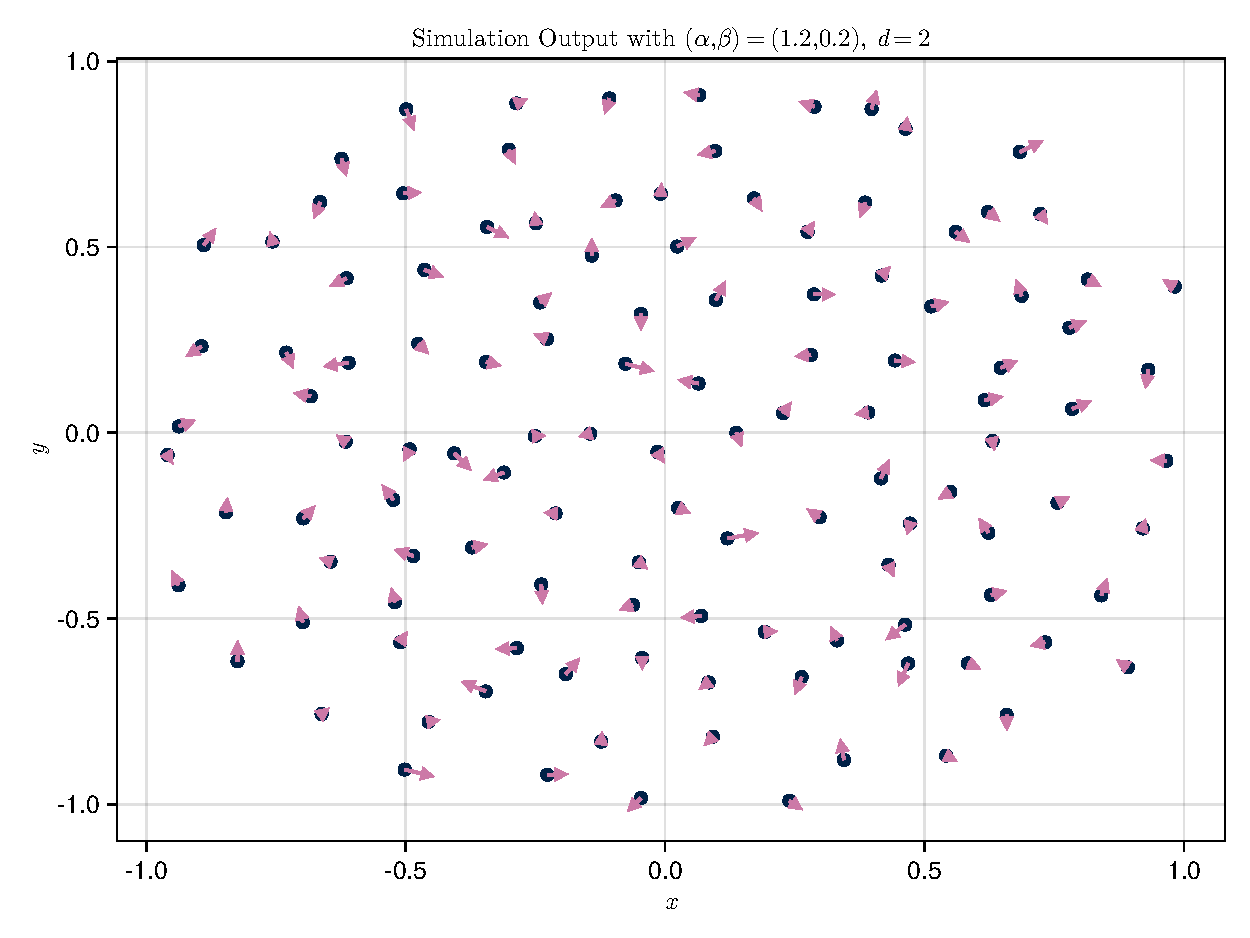
\includegraphics[width=0.8\linewidth]{results/simulation-quiver.pdf}
  \caption{Position and velocity of particles in the simulation.}
  % \paragraph{Link to Particle Simulator, give a Screenshot}
\end{figure}

\section{Continuous Limit}
% Introduce Continuous Limit, write about particle density \(\rho(x)\)
The total energy, in the continuous limit as $N_p \rightarrow \infty$, becomes
$$E = \frac{1}{2} \iint K\left(\norm{\vec{x} - \vec{y}}\right) \,\dd\rho(\vec{x})\,\dd\rho(\vec{y})\,,$$
where $\dd\rho = \rho(\vec{x})\dd\vec{x}$ is a measure (the equilibrium distribution) chosen such that
$$M = \int \dd\rho = \int_{\supp(\rho)} \rho(\vec{x}) \,\dd\vec{x} = 1\,.$$

\section{Self-Propulsion}
Makes it active matter.

Self-propulsion and friction could be modelled as a quadratic of the form
$$f(v_i) = 1.6 - 0.5 v_i^2\,,$$
where $v_i := \norm{\vec{v_i}} = \norm{\frac{\dd\vec{x_i}}{\ddt}}$.
Show reproduced plots from \cite{2006-self-propelled}.

% Friction Term -\textgreater{} Energy Dissipation -\textgreater{} Different Plot

\section{Kinetic Theory: The Vlasov Equation}
A very common tool in Plasma physics.
$$\frac{\partial f}{\partial t}+{\frac {\mathrm {d} \mathbf {r} }{\mathrm {d} t}}\cdot {\frac {\partial f}{\partial \mathbf {r} }}+{\frac {\mathrm {d} \mathbf {p} }{\mathrm {d} t}}\cdot {\frac {\partial f}{\partial \mathbf {p} }}=0,$$

This is the collisionless Boltzmann equation.
Vlasov replaces the collision term with long-range interactions.

\begin{theorem}{Liouville's}{liouville}
  Says that phase-space volume is conserved in situations of a pure particle-particle interaction.
  $$\frac{d\rho}{dt}=
    \frac{\partial\rho}{\partial t}
    +\sum_{i=1}^n\left(\frac{\partial\rho}{\partial q_i}\dot{q}_i
    +\frac{\partial\rho}{\partial p_i}\dot{p}_i\right)=0\,.$$
\end{theorem}

\section{Vicsek Model}
For the study of active matter (a number of individual agents).

\section{Swarming}
A 2010 paper by \citeauthor{2010-starlings} showed the surprising result that correlation between movement of individual starlings in bird flocks over Rome is scale-free.
In contrast to the assumption that birds only mirror their neighbours' behaviour and swarming behaviour emerges as a result of that, this observation suggests that bird flocks exert collective behaviour beyond local interactions.
\begin{quote}
  The change in the behavioral state of one animal affects and is affected by that of all other animals in the group, no matter how large the group is
  \parencite{2010-starlings}.
\end{quote}
This work was done by individually tracking each starling in the flock and using tracking algorithms to represent their 3 dimensional positions and velocities.
